\documentclass[tikz,border=3pt]{standalone}
\usepackage[T1]{fontenc}
\usepackage[scaled=0.95]{helvet}
\renewcommand{\familydefault}{\sfdefault}
\usepackage{amssymb}
\usetikzlibrary{arrows.meta,calc,decorations.pathmorphing}
\definecolor{cA}{HTML}{2a78d6}
\definecolor{cB}{HTML}{eb6834}
\definecolor{ink2}{HTML}{52514e}
\definecolor{mtop}{HTML}{d9dde2}
\definecolor{mtop2}{HTML}{cfd4da}
\definecolor{mfront}{HTML}{b3bac2}
\definecolor{mside}{HTML}{9aa2ab}
\begin{document}
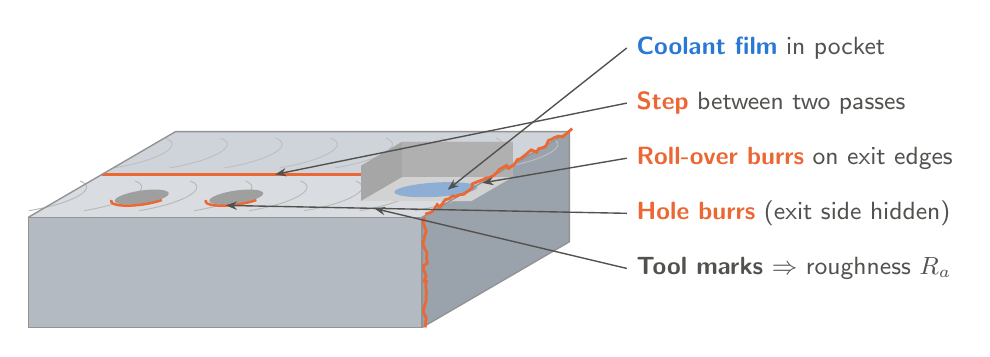
\begin{tikzpicture}[font=\sffamily\small,
  x={(1cm,0cm)}, y={(0cm,1cm)}, z={(0.55cm,0.32cm)},
  call/.style={-{Stealth[length=4pt]}, draw=ink2, line width=0.5pt},
  lab/.style={align=left, text=ink2}]
% faces
\fill[mfront] (0,0,0) -- (5,0,0) -- (5,1.4,0) -- (0,1.4,0) -- cycle;
\fill[mside]  (5,0,0) -- (5,0,3.4) -- (5,1.4,3.4) -- (5,1.4,0) -- cycle;
\fill[mtop]   (0,1.4,0) -- (5,1.4,0) -- (5,1.4,1.7) -- (0,1.4,1.7) -- cycle;
\fill[mtop2]  (0,1.4,1.7) -- (5,1.4,1.7) -- (5,1.4,3.4) -- (0,1.4,3.4) -- cycle;
% tool marks
\foreach \xc in {0.2,0.9,1.6,2.3,3.0,3.7,4.4,5.1} {
  \draw[gray!55, line width=0.35pt] plot[domain=-55:55, samples=20] ({\xc-0.75+0.72*cos(\x)},1.4,{0.85+0.72*sin(\x)});
  \draw[gray!50, line width=0.35pt] plot[domain=-55:55, samples=20] ({\xc-0.6+0.72*cos(\x)},1.4,{2.55+0.72*sin(\x)});
}
% step between passes
\draw[cB, line width=1.1pt] (0,1.4,1.7) -- (5,1.4,1.7);
% pocket
\fill[gray!55] (3.1,1.4,2.05) -- (4.5,1.4,2.05) -- (4.5,1.4,3.0) -- (3.1,1.4,3.0) -- cycle;
\fill[gray!70] (3.1,1.4,2.05) -- (3.1,1.4,3.0) -- (3.1,0.95,3.0) -- (3.1,0.95,2.05) -- cycle;
\fill[gray!62] (3.1,1.4,3.0) -- (4.5,1.4,3.0) -- (4.5,0.95,3.0) -- (3.1,0.95,3.0) -- cycle;
\fill[gray!35] (3.1,0.95,2.05) -- (4.5,0.95,2.05) -- (4.5,0.95,3.0) -- (3.1,0.95,3.0) -- cycle;
\fill[cA, opacity=0.4] plot[domain=0:360, samples=40, smooth cycle] ({3.8+0.5*cos(\x)},0.95,{2.5+0.3*sin(\x)});
% holes with entry burrs
\foreach \hx in {1.0,2.2} {
  \fill[gray!75] plot[domain=0:360, samples=40, smooth cycle] ({\hx+0.3*cos(\x)},1.4,{0.8+0.3*sin(\x)});
  \draw[cB, line width=0.9pt] plot[domain=200:340, samples=16, smooth] ({\hx+0.34*cos(\x)},1.4,{0.8+0.34*sin(\x)});
}
% outline
\draw[gray!85, line width=0.5pt] (0,0,0) -- (5,0,0) -- (5,1.4,0) -- (0,1.4,0) -- cycle;
\draw[gray!85, line width=0.5pt] (5,0,0) -- (5,0,3.4) -- (5,1.4,3.4) -- (5,1.4,0);
\draw[gray!85, line width=0.5pt] (0,1.4,0) -- (0,1.4,3.4) -- (5,1.4,3.4);
% exit-edge burrs
\draw[cB, line width=1.0pt, decorate, decoration={random steps, segment length=1.6pt, amplitude=0.9pt}] (5.04,1.44,0) -- (5.04,1.44,3.4);
\draw[cB, line width=1.0pt, decorate, decoration={random steps, segment length=1.6pt, amplitude=0.9pt}] (5.04,0,0) -- (5.04,1.4,0);
% callouts (all on the right)
\draw[call] (7.6,3.55) node[lab, anchor=west] {\textbf{\textcolor{cA}{Coolant film}} in pocket} -- (3.95,0.95,2.5);
\draw[call] (7.6,2.85) node[lab, anchor=west] {\textbf{\textcolor{cB}{Step}} between two passes} -- (2.2,1.4,1.7);
\draw[call] (7.6,2.15) node[lab, anchor=west] {\textbf{\textcolor{cB}{Roll-over burrs}} on exit edges} -- (5.05,1.42,1.3);
\draw[call] (7.6,1.45) node[lab, anchor=west] {\textbf{\textcolor{cB}{Hole burrs}} (exit side hidden)} -- (2.25,1.4,0.47);
\draw[call] (7.6,0.75) node[lab, anchor=west] {\textbf{Tool marks} $\Rightarrow$ roughness $R_a$} -- (4.2,1.4,0.35);
\end{tikzpicture}
\end{document}
